\newpage
\subsubsection{Skyscarper}
\label{Skyscarper}
Die Technik \textit{Skyscarper} bedeutet übersetzt Wolkenkratzer und leitet sich von der Anordnung der betrachteten Ziffern ab. Gesucht werden zwei Zeilen oder Spalten, in deren Kandidatenlisten die Ziffer jeweils noch genau zwei mal auftaucht. Wenn nun zwei der Kandidaten in der selben anderen Figur (Spalte oder Zeile) sind, dann hat man einen Wolkenkratzer gefunden. Die beiden Zahlen, die in der selben anderen Figur sind, bilden das Fundament des Wolkenkratzers, sie schließen sich gegenseitig aus. Das bedeutet wiederum, dass eine der beiden anderen gefundenen Ziffern dort stehen muss. Daher können alle Kandidaten, die von beiden Ziffern ausgeschlossen werden, aus den Kandidatenlisten gelöscht werden.	

\begin{figure}[h]
\begin{center}
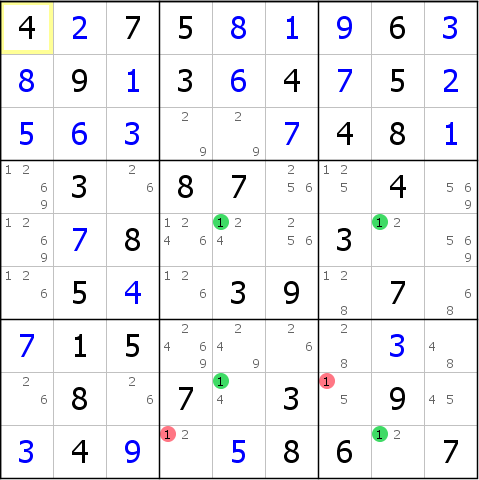
\includegraphics{./img/skyscarper.png}
\caption{Skyscarper}
\end{center}
\end{figure}

\noindent In \textbf{Abbildung 2.11} betrachten wir die Spalten 5 und 8. Hier sind die Bedingungen für den Wolkenkratzer erfüllt, da in jeder Spalte die Ziffer 1 jeweils genau zwei mal vorkommt und sie in beiden Spalten an Position 5 auftaucht. Für das Feld z9s8 gibt es nun zwei Möglichkeiten. Entweder die Ziffer 1 steht in diesem Feld oder nicht. Diese beiden Möglichkeiten werden nun separat betrachtet. Wenn die Ziffer 1 in Feld z9s8 steht, dann schließt das bereits alle rot markierten Zahlen aus. Für den Fall, dass die Ziffer 1 nicht in z9s8 steht, muss sie in z5s8 stehen, das geht aus der Bedingung des Wolkenkratzers hervor. Da sich nun z5s8 und z5s5 in der selben Zeile befinden, kann die Ziffer 1 nicht in z5s5 vorkommen. Deshalb muss sie in z8s5 stehen, wo sie alle rot markierten Felder ausschließt. In jeder Möglichkeit werden die roten Felder ausgeschlossen, daher kann die Ziffer 1 daraus gelöscht werden.